\message{ !name(main.tex)}\documentclass{article}
\usepackage{graphicx} % Required for inserting images
\usepackage{listings}
\graphicspath{ {images/} }

\title{}
\author{Vilhelm Lindell}
\date{August 2024}

\begin{document}

\message{ !name(main.tex) !offset(-3) }


\maketitle
\section{Introduction}
I detta gymnasiearbete är målet att undersöka och bygga en effektiv schackdator.
\section{Struktur}
För att representera en schackposition på ett sätt som är optimalt för datorn att hantera används så kallade Bitboards. En Bitboard är ett 64-bitar långt binärt tal, där varje bit representerar 1 ruta på shackbrädet. Anledningen till detta val är att programmet körs på och är optimiserat för en 64-bitars dator innebär det att vanliga operationer på 64-bitars tal är snabba. Eftersom att ett schackbräde har 64 rutor blir Bitboards användbara för att representera ockupation av rutor. En fördel med bitboards är att vi kan hitta positionen av den första biten som är 1, samt antalet bitar som är 1.

För att representera pjäsernas position har vi en bitboard per färg och pjäs, där vi låter bitar som är betyda att pjäsen finns på den rutan, och 0 att den inte finns på rutan.

Test



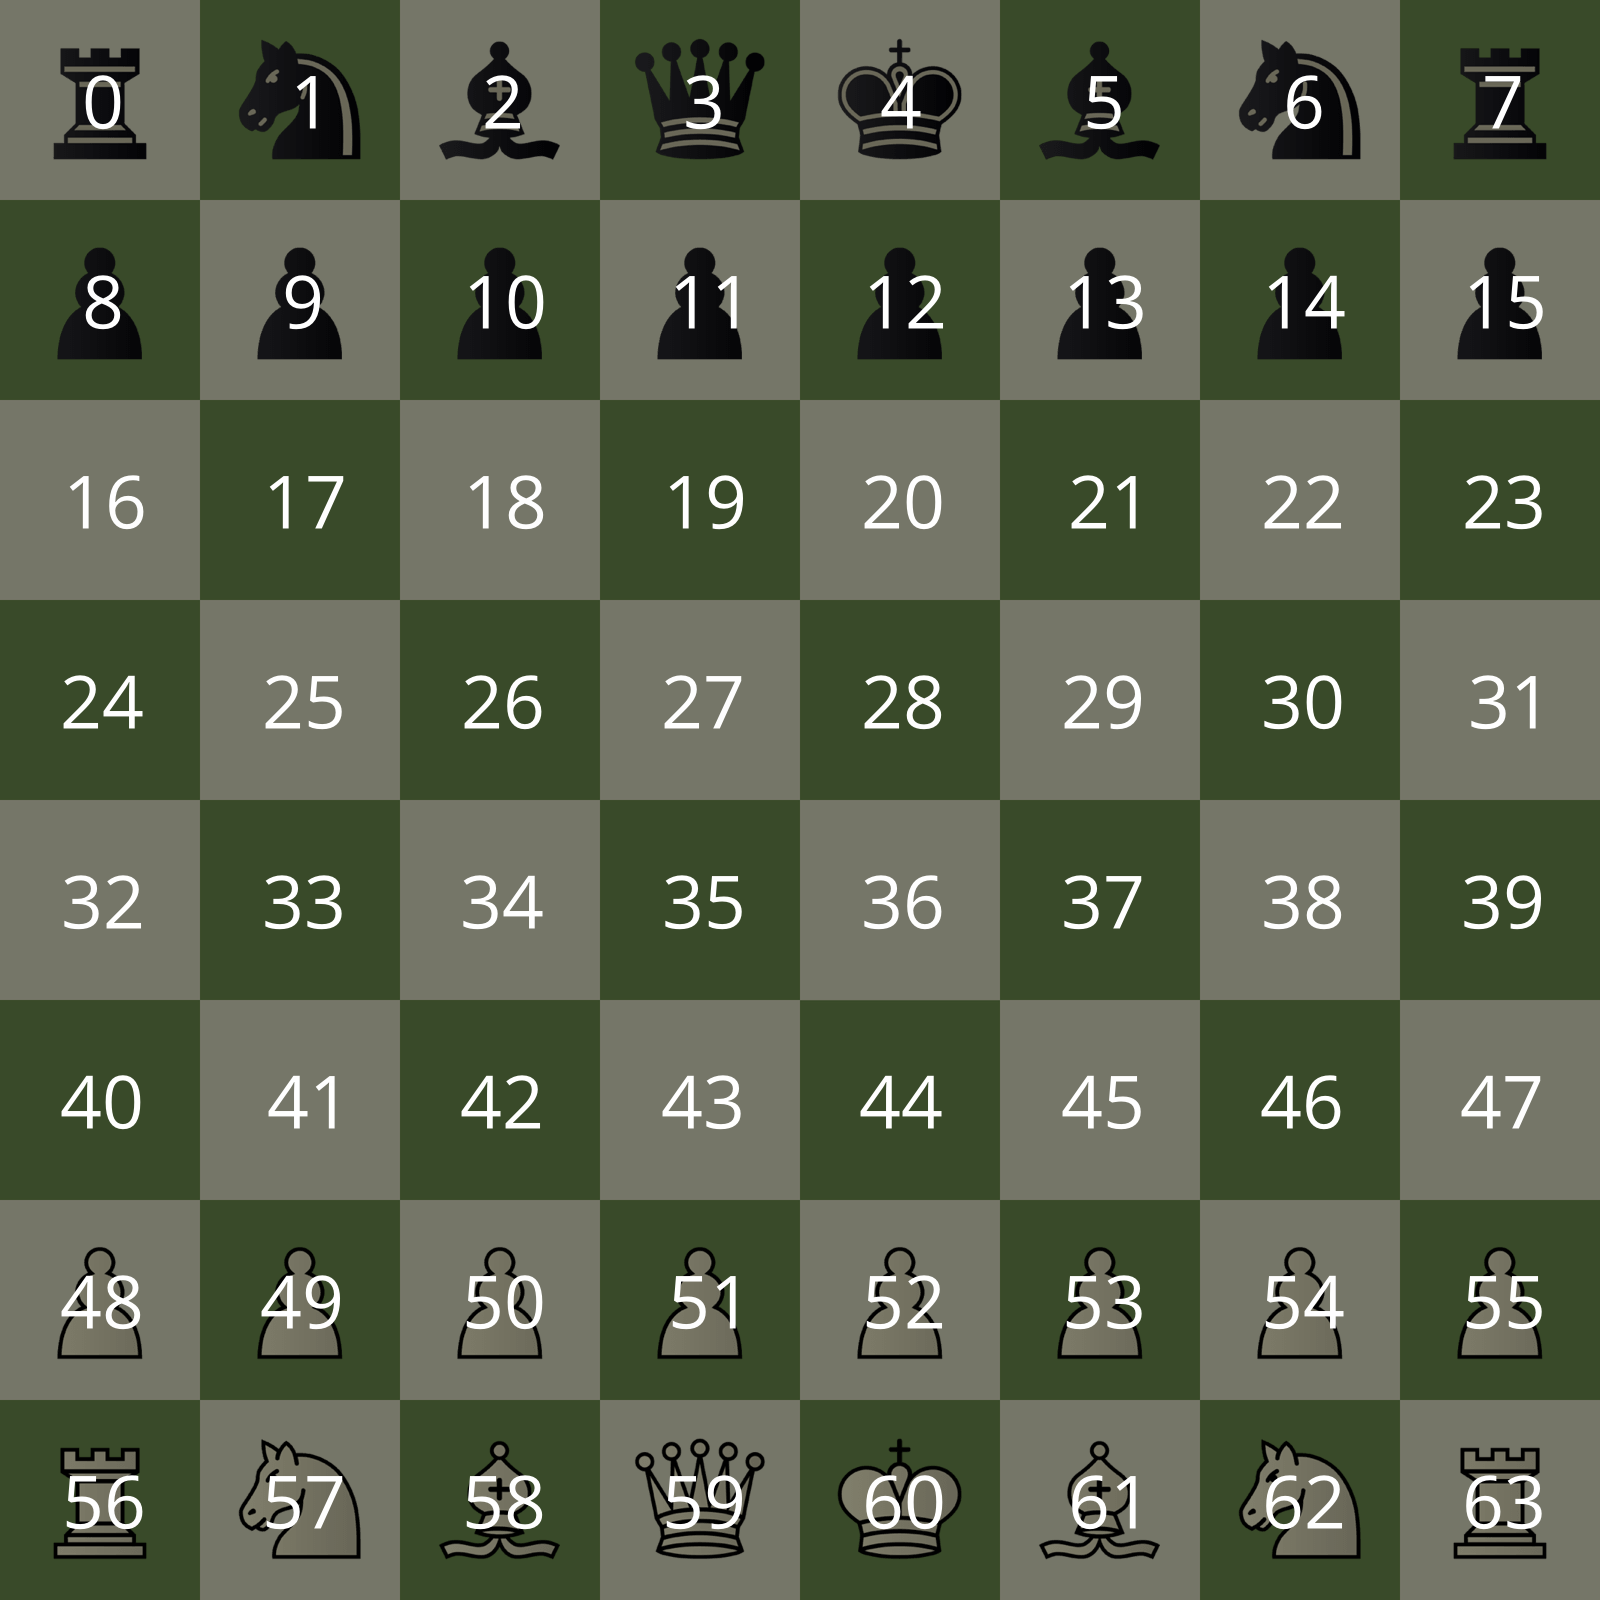
\includegraphics[scale=0.1]{board_indexed}

\begin{math}
a \ll k: 01100101 \ll 1 = 11001010
\end{math}

\section{Evaluering}
\section{Drag generering}


\section{Sökning}
Minimax är ett algoritm som används för att bestämma poängen efter ett visst mängd drag för ett noll-summa spel, med bästa drag enligt en evaluerings funktion. I mitt schackprogram använder jag en variation av minimax som kallas för negamax, vilket simplifierar koden genom att uttnytja följande faktum

\begin{math}
min(a,b)=max(-b,-a)
\end{math}

\subsection{Negamax}
Detta fungerar således evalueringsfunktionen returnerar ett värde som är relativt till sidan som gör draget--då större värden är bättre--vilket innebär att i negamax försöker både sidorna maximera evaluerings värde.

Algoritmen fungerar genom att gå igenom ett träd av alla möjliga positioner till ett visst djup. Vi börjar vid brädets nuvarande positionen och genererar en lista av alla lagliga drag. För varje lagligt drag skapar vi en ny nod i trädet som representerar schackbrädets position efter att draget har gjorts. Vi får ett heurestiskt värde för en av dessa barnnoder genom att anropa negamax igen från barnnoden, vilket kommer att ge oss ett heurestiskt värde för hur bra positionen är för den nuvarande spelaren.

Funktionen ger ett heurestiskt värde vid varje löv-nod som utgörs av de noder som nått det förutbestämda djupet eller som saknar lagliga drag, och noder som inte är löv-noder kommer ärva värdet värdet från det största värdet av sina barn noder. Funktionen kommer därmed rekursivt gå igenom trädet av alla drag på djupet först och varje nod kommer ärva det heurestiska värdet för det bässta draget i den nuvarande positionen.
Pseudokoden för algoritmet blir följande:

\begin{verbatim}
fn nega_max(depth ) {
    if (depth == 0) return evaluate();
    max = -oo;
    for (all moves)  {
        score = -negaMax(depth - 1);
        if(score > max)
            max = score;
    }
    return max;
}
\end{verbatim}

\subsection{Alpha-beta pruning}
Alpha-beta pruning är en förbättring på minimax som drastiskt kan minska antalet noder som behöver sökas. Principen utgår ifrån att vi sparar ett alfa och ett beta värde när vi söker, där alfa är det minsta poängen som den maximerande spelaren är garanterad, och beta är det största värdet som den minimerande spelaren är garanterad. Alfa får ett ursprungligt värde på -oo och beta oo. Dessa två värden är de sämsta möjliga som spelarna kan få, och när vi söker igenom trädet kommer vi uppdatera dessa. Efter vi har evaluerat värdet i en nod kollar vi ifall . Principen utgår ifrån att det bästa värdet som den maximerande spelaren kan få , a, är det sämsta värdet som den minimerande spelaren kan få, och tvärtom för b.

\subsection{Horisonteffekten}

Ett problem som dyker upp med vårt nuvarande sökalgoritm är en effekt som kallas för horisonteffekten. Eftersom vi har ett förutbestämt djup som vi söker till förekommer det situationer då det i lövnoden görs ett drag som har ett positivt vä. Ett exempel är ifall att det i en av lövnoderna görs ett drag där vits drottning tar en svart bonde, som i detta fallet blir positivt för vit. Problemet är att eftersom sökningen stannar vid detta djup kollar vi inte ifall det fanns en pjäs som skyddade den bonden och som nästa drag kommer ta drottningen. Detta kan lösas genom att vi inte stannar vid en nod som är instabil, dvs det finns drag som leder till en betydlig förändring i evalueringen. Det lättaste sättet att göra detta är att vi efter vår sökningen till en specifierad djuper, söker rekursivt genom alla drag som tar en annan pjäs. Detta fungerar relativt väl eftersom de drag som vanligast ger drastiska förändringar i evalueringen. Det finns fall där drag som inte tar pjäser ger drastiska förändringar i evalueringar, men dessa ignorerar vi att söka genom i vår horisontsökning eftersom det är svårt att bestämma det utan att göra draget, vilket skulle göra sökdjupet oändligt långt.

\subsection{Sortering av drag}

\

\begin{thebibliography}{9}

\end{thebibliography}

\end{document}

\message{ !name(main.tex) !offset(-82) }
